\section{Results}
\label{sec:results}

This section shows the results of our model performance and the user evaluation of our service implementation.

\subsection{Machine Learning}
\label{sec:learning}

We used the training data of 475 projects on three commonly used machine learning algorithms.
The projects varied in size and the algorithms we tested are: Logistic Regression, Naive Bayes and Random Forest.
We ran the three algorithms against each project with a 10-fold cross-validation.
The models were trained with 90\% of the training data, the remaining 10\% was used as test data.

In table~\ref{tab:alg-compare} it can be seen how the three algorithms performed.
Both LR and NB perform well on recall, but have a very low precision which makes it unusable for our application.
The RF algorithm performs less on recall, but achieves a higher precision, which is more important in our case.
High precision means that the algorithm returned substantially more relevant results than irrelevant.
It seems that RF is the best at identifying the important pull requests.

\begin{table}
  \begin{tabular}{lrrrrc}
    \hline
    \textbf{Algorithm} & \textbf{5\%} & \textbf{Mean} & \textbf{Median} & \textbf{95\%} & \textbf{Histogram} \\
    \hline

    \bf{Logistic Regression}\\
    Area Under Curve & 0.71 & 0.81 & 0.81 & 0.91 & \includegraphics[scale = 0.1, clip = true, trim= 50px 60px 50px 60px]{../figs/hist-results/hist-LRauc.pdf} \\
    Accuracy & 0.52 & 0.62 & 0.62 & 0.72 & \includegraphics[scale = 0.1, clip = true, trim= 50px 60px 50px 60px]{../figs/hist-results/hist-LRacc.pdf} \\
    Precision & 0.06 & 0.36 & 0.30 & 0.88 & \includegraphics[scale = 0.1, clip = true, trim= 50px 60px 50px 60px]{../figs/hist-results/hist-LRprec.pdf} \\
    Recall & 0.66 & 0.83 & 0.84 & 0.95 & \includegraphics[scale = 0.1, clip = true, trim= 50px 60px 50px 60px]{../figs/hist-results/hist-LRrec.pdf} \\
    F1 & 0.12 & 0.45 & 0.44 & 0.77 & \includegraphics[scale = 0.1, clip = true, trim= 50px 60px 50px 60px]{../figs/hist-results/hist-LRf1.pdf} \\

    \bf{Naive Bayes}\\
    Area Under Curve & 0.65 & 0.75 & 0.75 & 0.86 & \includegraphics[scale = 0.1, clip = true, trim= 50px 60px 50px 60px]{../figs/hist-results/hist-NBauc.pdf} \\
    Accuracy & 0.52 & 0.60 & 0.60 & 0.69 & \includegraphics[scale = 0.1, clip = true, trim= 50px 60px 50px 60px]{../figs/hist-results/hist-NBacc.pdf} \\
    Precision & 0.06 & 0.34 & 0.28 & 0.82 & \includegraphics[scale = 0.1, clip = true, trim= 50px 60px 50px 60px]{../figs/hist-results/hist-NBprec.pdf} \\
    Recall & 0.63 & 0.79 & 0.80 & 0.94 & \includegraphics[scale = 0.1, clip = true, trim= 50px 60px 50px 60px]{../figs/hist-results/hist-NBrec.pdf} \\
    F1 & 0.11 & 0.42 & 0.41 & 0.73 & \includegraphics[scale = 0.1, clip = true, trim= 50px 60px 50px 60px]{../figs/hist-results/hist-NBf1.pdf} \\

    \bf{Random Forest}\\
    Area Under Curve & 0.81 & 0.89 & 0.89 & 0.95 & \includegraphics[scale = 0.1, clip = true, trim= 50px 60px 50px 60px]{../figs/hist-results/hist-RFauc.pdf} \\
    Accuracy & 0.73 & 0.86 & 0.87 & 0.96 & \includegraphics[scale = 0.1, clip = true, trim= 50px 60px 50px 60px]{../figs/hist-results/hist-RFacc.pdf} \\
    Precision & 0.37 & 0.66 & 0.69 & 0.90 & \includegraphics[scale = 0.1, clip = true, trim= 50px 60px 50px 60px]{../figs/hist-results/hist-RFprec.pdf} \\
    Recall & 0.36 & 0.62 & 0.63 & 0.84 & \includegraphics[scale = 0.1, clip = true, trim= 50px 60px 50px 60px]{../figs/hist-results/hist-RFrec.pdf} \\
    F1 & 0.38 & 0.63 & 0.63 & 0.87 & \includegraphics[scale = 0.1, clip = true, trim= 50px 60px 50px 60px]{../figs/hist-results/hist-RFf1.pdf} \\
    \hline
  \end{tabular}
  \caption[Comparision of algorithms]{Comparision of algorithms. Scores and distributions of algorithm performance.}
  \label{tab:alg-compare}
\end{table}

The results in table~\ref{tab:alg-compare} led us believe that there was room for improvement.
Since the important snapshot data vs. unimportant data is very imbalanced, we decided to tune the balance.
However, balancing the data turned out to make things worse.

It is interesting to see that the age is a very dominant factor when we look at the feature importance in figure~\ref{fig:feature-importance}.
This is probably the case because it is very likely that new pull requests receive comments within the first few days.
Since the age feature is so dominant it could impact the model in a bad way.
When we turned this particular feature off, the results were worse instead.
So it seems the age has a positive effect on the prediction.

\begin{figure}
  \centering
  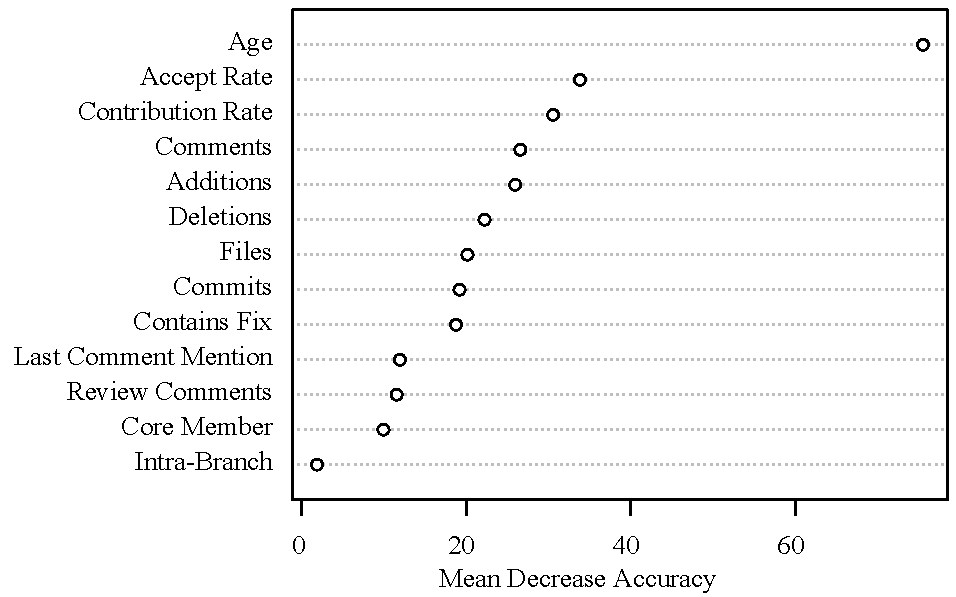
\includegraphics[width=0.45\textwidth]{../figs/mean-decrease-accuracy.pdf}
  \caption[Plot of feature importance]
   {Plot of feature importance of the aggregated projects. The age of the pull request is the dominant factor.}
  \label{fig:feature-importance}
\end{figure}

Despite the fact that it should be possible to further improve the prediction model and because this is only a preliminary study to prioritizing pull requests, we decided to go forward with the current model.

\subsection{Evaluation}
\label{sec:evaluation}

To test our service we invited a group of integrators that maintain open source projects.
The integrators were asked to answer statements on a scale with the following answers: strongly disagree, disagree, agree and strongly agree.
The values to the answers are ${-2, -1, 1, 2}$ respectively.
In addition to analysing their answers directly we also correlate the answers to the activity of their project.
We define the activity of their project as the average number of PR actions per day since the last 6 months.

The first questions were about the usefulness of certain features of the service.
Table~\ref{tab:usefulness} shows the averages of the given answers.
It can be seen that insight in the Contribution Rate, Test Code and Size are the most usefull features.

\resp{5}{The fact you can see how much the author of the pull request did in the past and how his success rate for getting pull requests in.
That is really useful information.
People that have a track record, will have obviously more chance to have their pull request looked at.}

However, the main highlight of the service, the Automatic Ordering, is on average neither positive nor negative rated.
This has probably something to do with the reasons why a certain PR is ranked higher than others (\respnum{6,7,9,17,19,20}).
\resp{17}{It can show us the most pressing pull requests.
However, it is unclear how this ranking is established, so I'd hope to know why a pull request is considered more urgent then others.}

Another thing that can be observed from table~\ref{tab:usefulness} is that the Target Branch and the Pairwise Conflicts features (the manual features) are rated more usefull for projects with more activity.

\begin{table}
  \center
  \begin{tabular}{lrr}
    \hline
    \textbf{Feature} & \textbf{Average} & \textbf{Activity correlation} \\
    \hline
    Contribution Rate  &  0.4286 &  0.1124 \\
    Has Test Code      &  0.3333 &  0.0186 \\
    Size               &  0.1905 &  0.3835 \\
    Pairwise Conflicts &  0.0952 &  0.4845 \\
    Automatic Ordering &  0.0000 & -0.0149 \\
    Target Branch      & -0.4762 &  0.6340 \\
    Accept Rate        & -0.0476 & -0.2268 \\
    \hline
  \end{tabular}
  \caption[Usefulness of features]{Usefulness of features. The average usefulness of the features and their correlation with the project activity.}
  \label{tab:usefulness}
\end{table}

The next part is about the usability of the service.
Around 86\% (18) says that using the service causes no extra overhead.
The given answers have a correlation of $0.4441$ with the activity of the project.

76\% (16) of the respondents thinks the prioritized overview of PRs is clear enough.
\resp{1}{I can see at a glance which PRs can be merged automatically.
For some reason the Github PR interface does not show this, you have to click on a PR to find out if it can be automatically merged.
In one of my projects, PRs often sit unmerged for a while and have to be rebased, so it's better to know when rebasing is necessary sooner, rather than later.}

Only 62\% (13) of the respondents agree that the set of used and presented fields is complete.
It seems that the integrators of more active projects tend to disagree, with a correlation of $-0.4054$.
This probably caused by the fact that the prioritization service lacks support for GitHub labels and milestones.

Later on in the questionaire we asked to rate some features for a next version of the prioritization service.
71\% (15) of the respondents indicated that they want to prioritize according to labels.
The correlation between the activity and the lack of label support is $0.4443$.
\resp{7}{I like the autosorting, but I'd like more control over it.
I use labels a lot for things, so for example, `needs followup' is a label that means I need to take no action, so I'd love to be able to tell you that.}

As said earlier, it is not clear for everyone on what grounds one pull request is higher ranked than others.
Almost all respondents (86\% or 18) want more control over the automatic ordering in a future version.
\resp{19}{It's very difficult to tell what the default ordering means.
This might be an inevitable consequence of machine learning but without some insight into why the results were ordered in a certain way (and maybe the ability to tweak the input weights), the view wasn't helpful.}

Finally we asked the respondents if they would use the prioritization service for their project.
57\% (12) of the respondent gave a positive answer.
With a activity correlation of $0.4307$ it seems that integrators with a more active project tend to use it more than those with less active projects.
\resp{15}{I actually don't find it very useful at all.
I've never had a problem prioritising pull requests, we keep the number of open pull requests below 30.
Generally, I respond to all pull requests raised on the project as soon as I receive the notification for them.}

The results are not very conclusive.
It seems that in its current form the automatic ordering is not adequate.
Users want to see why a PR is considered more important than others and have more control over the learning process.
On the other hand the manual sorting and filtering options are positively evaluated.
The Pairwise Conflicts, Target Branch and Size are the most popular.
Although the latter two are fairly trivial features GitHub's interface doesn't support them.
This might be the reason why the are rated usefull.
Finally, a narrow majority indicated that they will use the service for their project.
